% figure: ctrl-disturbance-block.png
% 用途：自控 03-5 稳态误差 —— 扰动作用下的闭环结构
% 构建：..\build.ps1 -File .\block-disturbance.tex
% 说明：旧图标签写作 G1(s)/G2(s)（非数学体）、蓝色方框与笔记其余插图不一致；
%       本图改用 TikZ，并改成与 03-8-1 一致的 G_1/G_2 记号。
\documentclass[border=10pt]{standalone}
\usepackage{fontspec}
\setmainfont{Cambria}
\usepackage{unicode-math}
\setmathfont{Cambria Math}
\usepackage{tikz}
\usetikzlibrary{positioning, arrows.meta, calc}
\usepackage{ctex}

\definecolor{figink}{HTML}{1E2228}
\definecolor{figacc}{HTML}{B23020}
\definecolor{figsub}{HTML}{606874}
\definecolor{figfill}{HTML}{E8EFF8}

\begin{document}
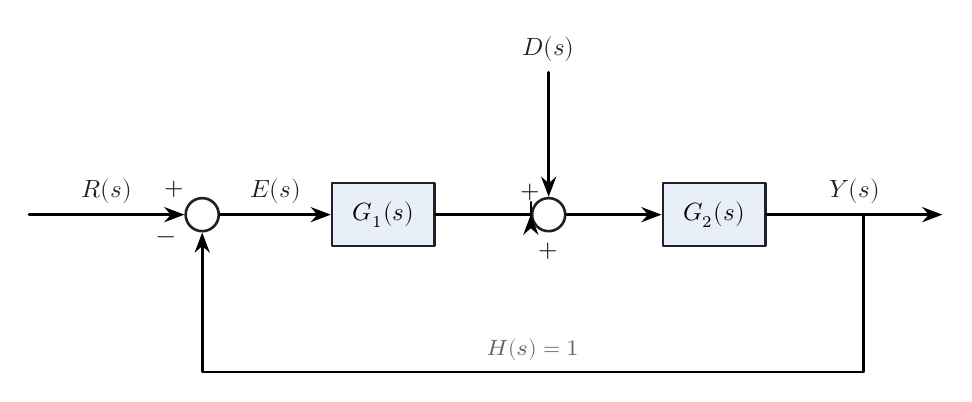
\begin{tikzpicture}[
  x=1cm, y=1cm,
  line width=0.95pt, line cap=round, line join=round,
  >=Stealth,
  blk/.style = {draw=figink, line width=0.95pt, fill=figfill,
                minimum width=1.3cm, minimum height=0.8cm, inner sep=2pt,
                anchor=center, font=\small},
  sum/.style = {draw=figink, line width=0.95pt, circle, inner sep=0pt,
                minimum size=0.42cm, anchor=center},
  sig/.style = {font=\small, color=figink},
  lbl/.style = {font=\small, inner sep=1.5pt},
  sub/.style = {font=\footnotesize, color=figsub}
]

\node[sum] (s1) at (0,0) {};
\node[blk] (g1) at (2.3,0) {$G_1(s)$};
\node[sum] (s2) at (4.4,0) {};
\node[blk] (g2) at (6.5,0) {$G_2(s)$};

% 输入与前向通道
\draw[->] (-2.2,0) -- node[sig, above] {$R(s)$} (s1.west);
\draw[->] (s1.east) -- node[sig, above] {$E(s)$} (g1.west);
\draw[->] (g1.east) -- (g1.east -| s2.west) -- (s2.west);
\draw[->] (s2.east) -- (g2.west);
\draw[->] (g2.east) -- node[sig, above] {$Y(s)$} (9.4,0);

% 扰动注入
\node[sig] (d) at (4.4,2.1) {$D(s)$};
\draw[->] (d) -- (s2.north);

% 单位负反馈
\draw[->] (8.4,0) -- (8.4,-2.0) -- (0,-2.0) -- (s1.south);
\node[sub] at (4.2,-1.72) {$H(s)=1$};

\node[lbl] at (-0.36,0.32) {$+$};
\node[lbl] at (-0.46,-0.32) {$-$};
\node[lbl] at (4.16,0.28) {$+$};
\node[lbl] at (4.4,-0.46) {$+$};

\end{tikzpicture}
\end{document}
